% Provenance (never printed): see sources/outline_sources.md (Year 2: index minerals and zones,
% geothermometers and geobarometers, prograde and retrograde paths, metamorphic series,
% ultrahigh-pressure rocks and exhumation, ocean-floor metamorphism). Garnet-biotite
% calibration refitted from the Ferry and Spear (1978) brackets tabulated by Holdaway et al.
% (1997); GASP from Koziol and Newton (1988); thickening model after England and Thompson
% (1984) in figdata/bachelor-2/ptpaths.py; exercise and problem values in the Book 4 scratch
% calculators calc/ch11.py and calc/ch11b.py.
\chapter{温压计与 P--T--t 轨迹}\label{ch:b2:pt-paths}

一颗在片岩中生长、直径仅几毫米的石榴子石，其核心保留着它开始生长时的成分，
边缘则保留着它停止生长时的成分。每一生长带当时都与其周围的黑云母和斜长石处于平衡，
而铁、镁、钙在这些矿物之间的分配
取决于温度和压力。结合上一章的热力学知识，石榴子石
可以告诉我们其所在岩石被埋藏得有多深、经历了多高的温度；
若对其定年，还能说明这一过程发生的时间，以及岩石\omterm{def:b2:pt-paths:exhumation}{折返}的速率。
本章将变质矿物转化为温度计、压力计
与时钟，并追踪一块岩石在地壳中的演化路径。

\begin{recall}
\textbf{高中分册}：变质级、指示矿物与等变质线。
\textbf{本科一年级分册}：地温线与放射性生热；
陆壳约 \qty{35}{km} 厚；放射性测年、矿物的封闭温度
及其给出的冷却年龄；洋壳及其\omterm{def:b2:mantle-melting:peridotites}{橄榄岩}。
\textbf{物理分册}：热传导方程 $\partial T/\partial t = \kappa\,
\partial^2 T/\partial z^2$ 与热扩散率 $\kappa$。\textbf{化学
分册}：平衡常数 $\Delta_r G^\circ + RT\ln K = 0$，以及
理想溶液中的活度。\textbf{见\cref{ch:b2:metamorphic-facies}}：\omterm{def:b2:metamorphic-facies:reaction}{变质反应}、
\omterm{def:b2:metamorphic-facies:clapeyron}{克拉珀龙斜率}、\ce{Al2SiO5} 相图与\omterm{def:b2:metamorphic-facies:facies}{变质相}。
\end{recall}
% ledger: prem:moho-average

\section{变质带}\label{sec:b2:pt-paths:zones}

1890 年代，乔治·巴罗在苏格兰高地的泥岩中划分出一系列
变质带，每一带以一种新指示矿物首次出现为标志。随变质级升高，
绿泥石之后依次出现黑云母、石榴子石、十字石、
蓝晶石和夕线石；在典型剖面中，石榴子石带至夕线石带形成于约 500 至
\qty{650}{\celsius}、5 至 \qty{7}{kbar} 的条件下。
% ledger: iugs:barrow, barrow1893:paper, earle:regional

\begin{definition}[巴罗带；变质场梯度]\label{def:b2:pt-paths:barrovian}
称\emph{巴罗带}\index{巴罗带}为\omterm{def:b2:metamorphic-facies:protoliths}{变泥质岩}中依次出现的变质带，
其顺序为绿泥石、黑云母、石榴子石、十字石、蓝晶石、夕线石，
每一带都始于其指示矿物的等变质线。某地区的\emph{变质场
梯度}\index{变质场梯度}是压力–温度平面上的一条曲线，
它穿过该地区各岩石在现今出露处
所记录的\omterm{def:b2:pt-paths:paths}{变质峰期条件}。
\end{definition}

\omterm{def:b2:pt-paths:barrovian}{变质场梯度}上的每一点都来自不同的岩石，每块岩石达到峰期的时间也各不相同，
因此\omterm{def:b2:pt-paths:barrovian}{变质场梯度}既不是某一时刻的地温线，也不是任何一块岩石的路径，
而是这些峰期条件在现今剥蚀面上留下的痕迹。

\begin{omfigure}
\centering
\begin{tikzpicture}[x=1cm, y=1cm]
\def\iso{{0,1.9,3.7,5.5,7.3,9.1,11}}
\foreach \i [evaluate=\i as \op using 4+9*\i] in {0,...,5} {
  \pgfmathsetmacro{\xa}{\iso[\i]}\pgfmathsetmacro{\xb}{\iso[\i+1]}
  \pgfmathsetmacro{\da}{(\i>0)*0.2}\pgfmathsetmacro{\db}{(\i<5)*0.2}
  \fill[red!\op!white] (\xa-\da,0) -- (\xb-\db,0) -- (\xb+\db,4) -- (\xa+\da,4) -- cycle;
}
\foreach \x/\n in {1.9/黑云母, 3.7/石榴子石, 5.5/十字石, 7.3/蓝晶石, 9.1/夕线石} {
  \draw[very thick, red!70!black] (\x-0.2,0) -- (\x+0.2,4);
  \node[font=\scriptsize, red!70!black, anchor=south] at (\x+0.2,4.05) {\n};
}
\draw[thick] (0,0) rectangle (11,4);
\foreach \x/\z in {0.95/绿泥石, 2.8/黑云母, 4.6/石榴子石, 6.4/十字石, 8.2/蓝晶石, 10.05/夕线石}
  \node[font=\scriptsize\itshape, align=center] at (\x,2) {\z\\带};
\draw[->, thick] (0.4,-0.35) -- node[below, font=\scriptsize] {变质级升高} (10.6,-0.35);
\end{tikzpicture}
\par\smallskip{\small \omterm{def:b2:pt-paths:barrovian}{巴罗带}示意图（平面图，示意）。每条等变质线（红线，图上方标注其名称）
是其指示矿物首次出现的位置；
变质级与阴影深度向右增加。每个带以
其低级边界处出现的矿物命名。}
\end{omfigure}
% ledger: iugs:barrow

等变质线由矿物出现的位置测绘而来，
只有弄清其背后的反应之后，才能成为压力和温度的条件。
要进一步研究，需要在同一块岩石中同时测量温度和压力。

\section{温度计与压力计}\label{sec:b2:pt-paths:thermobarometry}

\begin{definition}[地质温度计；地质压力计；交换反应；净转移反应]\label{def:b2:pt-paths:thermobarometry}
称\emph{地质温度计}\index{地质温度计}（\emph{地质压力计}\index{地质压力计}）为
矿物间的一种平衡，其位置主要取决于温度（压力），
因而矿物的成分可给出其最后一次平衡时的温度（压力）。
两种矿物之间交换两种元素的反应称\emph{交换反应}\index{交换反应}，
例如石榴子石与黑云母之间交换铁和镁，
且不产生也不消耗任何一种矿物。\emph{净转移反应}\index{净转移反应}则是
某些矿物以另一些矿物为代价而生成。
\end{definition}

\omterm{def:b2:metamorphic-facies:protoliths}{变泥质岩}中应用最广的温度计，是石榴子石与黑云母之间的
铁、镁交换，
\[
\ce{Fe3Al2Si3O12 + KMg3AlSi3O10(OH)2 <=> Mg3Al2Si3O12 + KFe3AlSi3O10(OH)2},
\]
由铁铝榴石与金云母生成镁铝榴石与铁云母。设 $X_{\text{Mg}}$ 与 $X_{\text{Fe}}$
分别为每种矿物中由镁和铁占据的位置分数，并记
\[
K_D = \frac{(X_{\text{Mg}}/X_{\text{Fe}})_{\text{石榴子石}}}{(X_{\text{Mg}}/X_{\text{Fe}})_{\text{黑云母}}}.
\]
% ledger: h97:fs-reaction

\begin{proposition}[一个交换平衡]\label{prop:b2:pt-paths:exchange}
若石榴子石与黑云母为理想溶液，且上述反应的 $\Delta_r H$、$\Delta_r S$ 与 $\Delta_r V$
均为常数，则在平衡时
\[
3RT\ln K_D = -(\Delta_r H + P\,\Delta_r V) + T\,\Delta_r S,
\qquad\text{故}\qquad
T = \frac{\Delta_r H + P\,\Delta_r V}{\Delta_r S - 3R\ln K_D}.
\]
\end{proposition}

\begin{proof}
每种矿物都有三个供铁或镁占据的位置。理想溶液中，端元组分的活度
等于其所占位置分数的乘积：$a_{\text{镁铝榴石}} =
X_{\text{Mg}}^3$（石榴子石中），依此类推。于是平衡常数为
\[
K = \frac{a_{\text{镁铝榴石}}\,a_{\text{铁云母}}}{a_{\text{铁铝榴石}}\,a_{\text{金云母}}}
= \frac{X_{\text{Mg,grt}}^3\,X_{\text{Fe,bt}}^3}{X_{\text{Fe,grt}}^3\,X_{\text{Mg,bt}}^3} = K_D^3 .
\]
平衡时 $\Delta_r G^\circ(T, P) + RT\ln K = 0$，其中 $\Delta_r G^\circ = \Delta_r H -
T\,\Delta_r S + P\,\Delta_r V$（略去 $P - 1$ 中的 1），由此即得第一式；
解出 $T$ 即得第二式。
\end{proof}

这些常数来自人工合成石榴子石与黑云母交换铁、镁的实验，
实验温度已知，压强为 \qty{2.07}{kbar}。共十二组此类夹逼实验，温度自 550 至
\qty{800}{\celsius}，以 $\ln K_D$ 对 $1/T$ 作图，近似落在一条直线上
（见下图）；用最小二乘法拟合，取 $\Delta_r V = \qty{0.311}{J.bar^{-1}}$，
得 $\Delta_r H = \qty{52630}{J}$ 与 $\Delta_r S = \qty{20.19}{J.K^{-1}}$，这些值与
同一批数据已发表的重算值相符。温度升高时，比值 $K_D$ 趋向 1：
石榴子石占有更多的镁。
% ledger: h97:fs-data, h97:ideal, h97:fs-reaction

\begin{omfigure}
\centering
\begin{tikzpicture}
\begin{axis}[omrecord, width=0.62\linewidth, height=5.2cm,
  xmin=0.9, xmax=1.25, ymin=-1.9, ymax=-1.1,
  xlabel={$1000/T$ (\unit{K^{-1}})}, ylabel={$\ln K_D$},
  tick label style={font=\scriptsize}, label style={font=\small},
  x tick label style={/pgf/number format/.cd, fixed, precision=2}]
\addplot[only marks, mark=*, mark size=1.6pt, blue!70!black]
  table[x expr={1000/(\thisrow{T_C}+273.15)}, y=lnKD] {figdata/out/bachelor-2-ptpaths-fs.dat};
\addplot[thick, red!75!black, domain=0.9:1.25, samples=2] {(-52630-2070*0.311)/(3*8.31441)*x/1000 + 20.19/(3*8.31441)};
\end{axis}
\end{tikzpicture}
\par\smallskip{\small 石榴子石–黑云母交换：十二组实验夹逼点，
压强 \qty{2.07}{kbar} 下（蓝色，据 Holdaway 等人，1997 年列表），以及
由命题及拟合所得 $\Delta_r H$、$\Delta_r S$ 确定的直线（红色）。}
\end{omfigure}
% ledger: h97:fs-data, h97:ideal

当 $K_D = 0.18$ 且压强为 \qty{5}{kbar} 时，$T = (52630 + 0.311\times5000)/(20.19 - 3\times8.314
\times\ln 0.18) = 54185/62.96 = \qty{861}{K}$，合 \qty{587}{\celsius}。压强每增加 1 kbar
约使温度增加 $0.311\times1000/62.96 = \qty{4.9}{K}$：该反应使电荷相同的离子
在大小相近的位置之间交换，体积变化很小，压强几乎无影响。
这正是它可以用作温度计的原因。

气压计则需要相反的情形：体积变化很大的反应。以下\omterm{def:b2:pt-paths:thermobarometry}{净转移
反应}
\[
\ce{3 CaAl2Si2O8 <=> Ca3Al2Si3O12 + 2 Al2SiO5 + SiO2},
\]
钙长石生成钙铝榴石、蓝晶石与石英，将三份长石的原子
压入更致密的矿物中：$\Delta_r V = \qty{-6.21}{J.bar^{-1}}$，其绝对值为\omterm{def:b2:pt-paths:thermobarometry}{交换反应}的二十倍。
其端元平衡经实验逆转，条件为 900 至 \qty{1250}{\celsius}、19
至 \qty{28}{kbar}，平衡线为
\[
P_0 = 22.80\,T - 1093 \qquad (P_0 \text{ 单位为 bar}, T \text{ 单位为 } \unit{\celsius}).
\]
在岩石中，钙铝榴石只是石榴子石的一小部分，钙长石是
斜长石的一部分。理想活度下，$a_{\text{钙铝榴石}} = X_{\text{Ca,grt}}^3$ 与
$a_{\text{钙长石}} = X_{\text{an}}$，取条件 $\Delta_r G^\circ + RT\ln K = 0$
分别在 $P$ 与 $P_0$ 处写出，得
\[
P = P_0 + \frac{RT}{6.21}\,\ln\frac{X_{\text{Ca,grt}}^3}{X_{\text{an}}^3}
\qquad (T \text{ 在第二项中以开尔文为单位}).
\]
这一\omterm{def:b2:pt-paths:thermobarometry}{地质压力计}以四种矿物命名为 GASP（石榴子石、铝硅酸盐、二氧化硅、
斜长石），适用于凡含这四种矿物的\omterm{def:b2:metamorphic-facies:protoliths}{变泥质岩}。
% ledger: kn88:gasp, rh95:gb-gasp

\begin{method}[单个岩石的温度与压力]\label{met:b2:pt-paths:intersection}
（1）在共生矿物中测定温度计和压力计所需的成分。
（2）假定一个压强，用温度计算温度。
（3）在该温度下，用压力计算压强。（4）重复（2）与（3），
直至两者都不再改变；通常两三轮即可，因为每个方程对另一式所固定的
变量依赖较弱。图解上，答案即温度计的直线
与压力计直线的交点。（5）传递不确定度：对独立误差，
$\sigma_T^2 = (\partial T/\partial\ln K_D)^2\sigma_{\ln K_D}^2 +
(\partial T/\partial P)^2\sigma_P^2$，对 $P$ 同理。
\end{method}

\begin{omfigure}
\centering
\begin{tikzpicture}
\begin{axis}[omrecord, width=0.78\linewidth, height=6.4cm,
  xmin=400, xmax=800, ymin=0, ymax=12, xlabel={$T$ (\unit{\celsius})}, ylabel={$P$ (\unit{kbar})},
  tick label style={font=\scriptsize}, label style={font=\small}, clip=false]
\addplot[thick, red!75!black] table[x=kd12, y=P_kbar] {figdata/out/bachelor-2-ptpaths-gb.dat};
\addplot[thick, red!75!black] table[x=kd15, y=P_kbar] {figdata/out/bachelor-2-ptpaths-gb.dat};
\addplot[thick, red!75!black] table[x=kd18, y=P_kbar] {figdata/out/bachelor-2-ptpaths-gb.dat};
\addplot[thick, red!75!black] table[x=kd21, y=P_kbar] {figdata/out/bachelor-2-ptpaths-gb.dat};
\addplot[thick, red!75!black] table[x=kd24, y=P_kbar] {figdata/out/bachelor-2-ptpaths-gb.dat};
\addplot[thick, blue!70!black] table[x=T_C, y=r15] {figdata/out/bachelor-2-ptpaths-gasp.dat};
\addplot[thick, blue!70!black] table[x=T_C, y=r20] {figdata/out/bachelor-2-ptpaths-gasp.dat};
\addplot[thick, blue!70!black] table[x=T_C, y=r25] {figdata/out/bachelor-2-ptpaths-gasp.dat};
\addplot[thick, blue!70!black] table[x=T_C, y=r30] {figdata/out/bachelor-2-ptpaths-gasp.dat};
\node[font=\tiny, red!75!black, anchor=west] at (axis cs:452,0.5) {0.12};
\node[font=\tiny, red!75!black, anchor=west] at (axis cs:511,0.5) {0.15};
\node[font=\tiny, red!75!black, anchor=west] at (axis cs:568,0.5) {0.18};
\node[font=\tiny, red!75!black, anchor=west] at (axis cs:622,0.5) {0.21};
\node[font=\tiny, red!75!black, anchor=west] at (axis cs:675,0.5) {0.24};
\node[font=\tiny, blue!70!black, anchor=west] at (axis cs:802,8.97) {0.15};
\node[font=\tiny, blue!70!black, anchor=west] at (axis cs:802,10.21) {0.20};
\node[font=\tiny, blue!70!black, anchor=west] at (axis cs:802,11.17) {0.25};
\node[font=\tiny, blue!70!black, anchor=west] at (axis cs:802,11.96) {0.30};
\end{axis}
\end{tikzpicture}
\par\smallskip{\small 石榴子石–黑云母等温线（红色、较陡，以 $K_D$ 标注）与 GASP
等压线（蓝色，右侧标注比值 $X_{\text{Ca}}/X_{\text{an}}$，即
石榴子石中钙铝榴石与斜长石中钙长石之比）。据本节标定，含两对矿物的岩石
位于两条线的交点处。}
\end{omfigure}
% ledger: h97:ideal, h97:fs-reaction, kn88:gasp

等温线几乎竖直，等压线倾斜，二者以较大夹角相交，
这使交点的定位较为精确。理想混合是本章的主要简化。
真实的石榴子石含有钙和锰，真实的黑云母含有铝、
钛和三价铁；对这些成分加以修正的标定会使温度改变数十摄氏度（在某一研究较充分的地区，
为 \qty{574}{\celsius} 而非 \qty{530}{\celsius}）；
最好的标定声称不确定度约为 \qty{25}{\celsius}。
% ledger: h97:ideal, h97:corrections

\section{压强–温度轨迹}\label{sec:b2:pt-paths:paths}

一块岩石并不会在同一时刻达到最高压强和最高温度。
它先被埋藏并加热，随后被抬升并冷却，
其矿物在此过程中始终发生反应。

\begin{definition}[P--T 轨迹；进变质轨迹与退变质轨迹；变质峰期条件]\label{def:b2:pt-paths:paths}
岩石的\emph{P--T 轨迹}\index{P--T 轨迹}是其在一次变质事件中
经历的压强与温度序列。其\emph{进变质轨迹}\index{进变质轨迹}
是温度上升的那一段，其\emph{退变质轨迹}\index{退变质轨迹}
则是温度下降的那一段。\emph{变质峰期条件}\index{变质峰期条件}
是轨迹上温度最高处的压强与温度，即热峰；
压强峰，又称压力峰，
未必与之重合。
\end{definition}
% ledger: scmr:ptt

若轨迹以温度为横轴（向右）、压强为纵轴（向上）绘出，
且热峰出现在压强峰之后、即减压过程中，则称该轨迹为\emph{顺时针}的；
若热峰到达时压强仍在上升，则为\emph{逆时针}的。岩石沿哪种方向，
取决于热量如何到达它，
其中最简单的情形可以算出。
% ledger: scmr:ptt

设想一地壳厚 \qty{35}{km}，处于稳态，放射性生热率为
\qty{1.0}{\micro W.m^{-3}}，自下方传入的热流为 \qty{25}{mW.m^{-2}}，传导率为
\qty{2.5}{W.m^{-1}.K^{-1}}，热扩散率为 \qty{1e-6}{m^2.s^{-1}}，后三者均取自岩石实测范围之内。
其地表热流为 \qty{60}{mW.m^{-2}}，莫霍面处温度为
\qty{595}{\celsius}。碰撞使该地壳的第二份叠置于其上，相对热量传导所需的时间而言，此过程很快：
下层岩片的岩石保持原有温度，但深度增加了 \qty{35}{km}，
地温线因而呈锯齿状，
\qty{35}{km} 深处温度为 \qty{0}{\celsius} 的岩石位于上层热岩石之下。地壳
现厚 \qty{70}{km}，所含放射性生热岩石为原来的两倍。叠置后三千万年，
侵蚀开始，在 7000 万年内剥蚀掉 \qty{35}{km}
（\qty{0.5}{mm.\text{年}^{-1}}）。
% ledger: delaney:conductivity, roy:granitic-k, vila:heat-production, prem:moho-average, et84:ptt

\begin{proposition}[热弛豫的时间尺度]\label{prop:b2:pt-paths:relaxation}
在厚度为 $L$ 的层中，若其两个界面保持恒定温度，则
形如 $\sin(\pi z/L)$ 的温度干扰按 $e^{-t/\tau}$ 衰减，其中
\[
\tau = \frac{L^2}{\pi^2\kappa}.
\]
\end{proposition}

\begin{proof}
设 $\theta(z, t) = f(t)\sin(\pi z/L)$，它在 $z = 0$ 与 $z = L$ 处为零。热传导
方程 $\partial\theta/\partial t = \kappa\,\partial^2\theta/\partial z^2$ 给出
$f'\sin(\pi z/L) = -\kappa(\pi/L)^2 f\sin(\pi z/L)$，故 $f' = -f/\tau$，其中 $\tau =
L^2/(\pi^2\kappa)$，且 $f = f(0)\,e^{-t/\tau}$。
\end{proof}

锯齿形的波长与单层厚度同量级：取 $L =
\qty{35}{km}$，$\tau = \qty{3.9}{Ma}$，\qty{35}{km} 深处的冷楔
在 1000 万年内即被抹平。整个加厚地壳 $L = \qty{70}{km}$ 的弛豫时间为 $\tau =
\qty{16}{Ma}$，因此加热会持续数千万年，趋向于
厚度加倍、放射性生热岩石也加倍的地壳所能维持的
高得多的地温线。下图
给出所计算的地温线。
% ledger: delaney:conductivity

\begin{omfigure}
\centering
\begin{tikzpicture}
\begin{axis}[omrecord, width=0.62\linewidth, height=6.6cm,
  xmin=0, xmax=1000, ymin=0, ymax=80, y dir=reverse,
  xlabel={$T$ (\unit{\celsius})}, ylabel={深度 (\unit{km})},
  legend style={font=\scriptsize, at={(0.02,0.02)}, anchor=south west},
  tick label style={font=\scriptsize}, label style={font=\small}]
\addplot[thick, black] table[x=t0, y=z_km] {figdata/out/bachelor-2-ptpaths-geo.dat};
\addlegendentry{\qty{0}{Ma}}
\addplot[thick, blue!70!black] table[x=t10, y=z_km] {figdata/out/bachelor-2-ptpaths-geo.dat};
\addlegendentry{\qty{10}{Ma}}
\addplot[thick, orange!85!black] table[x=t30, y=z_km] {figdata/out/bachelor-2-ptpaths-geo.dat};
\addlegendentry{\qty{30}{Ma}}
\addplot[thick, red!75!black] table[x=t60, y=z_km] {figdata/out/bachelor-2-ptpaths-geo.dat};
\addlegendentry{\qty{60}{Ma}}
\end{axis}
\end{tikzpicture}
\par\smallskip{\small 将 \qty{35}{km} 地壳通过叠置加倍后的地温线，
用热传导方程计算（深度均自当时地表算起；侵蚀始于
\qty{30}{Ma}）。黑线：叠置刚结束时的锯齿形地温线。加厚地壳的底部，
起初为 \qty{595}{\celsius}，6000 万年后超过 \qty{900}{\celsius}。}
\end{omfigure}
% ledger: et84:ptt

追踪叠置前位于地表、叠置后恰位于 \qty{35}{km} 深处的岩石，其
位于 \qty{9.6}{kbar} 之下。500 万年内，它在不发生位移的情况下从 0 升温至
\qty{395}{\celsius}；至侵蚀开始时，已达到
\qty{558}{\celsius}。随后侵蚀将其抬升，但热量的到达速度始终快于其
散失速度：岩石在抬升 \qty{6}{km} 时仍在升温，并达到其热峰，
即 \qty{593}{\celsius}、\qty{7.8}{kbar}，叠置后 4300 万年。此后
岩石才开始冷却，经过 \qty{405}{\celsius}，深度为 \qty{13}{km}，
时间为 \qty{74}{Ma}，此后向地表抬升。下图中的轨迹为顺时针方向。此外，
它在其峰值温度 \qty{50}{\celsius} 范围内停留了三千万年，约占其整个历程的
三分之一。英格兰与汤普森于 1984 年发现，对于大多数地质上可信的
情形，岩石会长时间接近其峰值，所保存的矿物
主要记录的是这一阶段。
% ledger: et84:ptt

\begin{omfigure}
\centering
\begin{tikzpicture}
\begin{axis}[omrecord, width=0.78\linewidth, height=6.2cm,
  xmin=0, xmax=800, ymin=0, ymax=11, xlabel={$T$ (\unit{\celsius})}, ylabel={$P$ (\unit{kbar})},
  tick label style={font=\scriptsize}, label style={font=\small}]
\addplot[thick, gray, densely dashed, restrict x to domain=0:504] table[x=T_C, y=P_kbar] {figdata/out/bachelor-2-facies-hm93-kyand.dat};
\addplot[thick, gray, densely dashed] table[x=T_C, y=P_kbar] {figdata/out/bachelor-2-facies-hm93-kysil.dat};
\addplot[thick, gray, densely dashed] table[x=T_C, y=P_kbar] {figdata/out/bachelor-2-facies-hm93-andsil.dat};
\addplot[very thick, red!75!black, postaction={decorate}, decoration={markings,
  mark=at position 0.2 with {\arrow{Stealth[length=2.5mm]}},
  mark=at position 0.52 with {\arrow{Stealth[length=2.5mm]}},
  mark=at position 0.8 with {\arrow{Stealth[length=2.5mm]}}}] table[x=T_C, y=P_kbar] {figdata/out/bachelor-2-ptpaths-path.dat};
\node[font=\scriptsize\bfseries, gray] at (axis cs:330,6.5) {蓝晶石};
\node[font=\scriptsize\bfseries, gray] at (axis cs:520,1.0) {红柱石};
\node[font=\scriptsize\bfseries, gray] at (axis cs:740,4.0) {夕线石};
\node[font=\scriptsize, red!75!black, anchor=south] at (axis cs:200,9.7) {深部加热};
\node[font=\scriptsize, red!75!black, anchor=west] at (axis cs:603,8.9) {热峰};
\node[font=\scriptsize, red!75!black, anchor=west] at (axis cs:110,2.7) {冷却抬升};
\end{axis}
\end{tikzpicture}
\par\smallskip{\small 叠置后恰位于 \qty{35}{km} 深处的岩石的 \omterm{def:b2:pt-paths:paths}{P--T 轨迹}
（红色，每两百万年取样一次），用上图地温线模型计算，
叠加于\cref{ch:b2:metamorphic-facies}中的 \ce{Al2SiO5} 实验相图之上（灰色）。
压强峰先出现，热峰则出现在减压过程中：此为顺时针轨迹，
始终未离开蓝晶石域。}
\end{omfigure}
% ledger: et84:ptt, hm93:table11

模型还说明了为何有些轨迹走向相反。单纯增厚只会在岩石被埋藏后才使其升温，
因此其热峰出现在\omterm{def:b2:pt-paths:exhumation}{折返}期间。若岩石在仍被埋藏时温度即已上升，
则需要外部热源，例如\omterm{def:b2:magma-emplacement:magma}{岩浆}上升侵入其上方或旁侧的地壳，
轨迹即为逆时针。在增厚的地壳中，底部温度远高于其初始值，
英格兰与汤普森得出结论，地壳的大量熔融是增厚
很可能带来的结果，
这正是\cref{ch:b2:crustal-melting}的主题。
% ledger: et84:ptt, scmr:ptt

\section{添加时间}\label{sec:b2:pt-paths:time}

\begin{definition}[P--T--t 轨迹]\label{def:b2:pt-paths:ptt}
岩石的\emph{P--T--t 轨迹}\index{P--T--t 轨迹}，即其 \omterm{def:b2:pt-paths:paths}{P--T 轨迹}，并
标注各点到达的时间。
\end{definition}
% ledger: scmr:ptt

时间由放射性测年给出。一种在该事件中生长、此后一直保留子体同位素的矿物，
例如用钐—钕法定年的石榴子石环带，可测得其自身的生长年龄，
其成分则给出
该时刻的压强和温度。较早形成、温度更高时生长的矿物，
则给出冷却年龄：岩石冷却至
该矿物与同位素体系的封闭温度的时刻（本科一年级分册）。
以半径为 \qty{100}{\micro m} 的白云母颗粒中的氩为例，冷却速率为
每百万年 \qty{10}{\celsius}，封闭温度在
\qty{5}{kbar} 时为 \qty{405}{\celsius}，在 \qty{10}{kbar} 时为 \qty{425}{\celsius}。
% ledger: h09:muscovite

\begin{definition}[折返；折返速率]\label{def:b2:pt-paths:exhumation}
\emph{折返}\index{折返}是指岩石向地表的运动，通过
移除其上覆岩石实现。\emph{折返速率}\index{折返速率}是
其深度的减小速率。
\end{definition}

\begin{proposition}[由两个定年点求速率]\label{prop:b2:pt-paths:rates}
若岩石处于温度 $T_1$、深度 $z_1$ 的时刻为 $t_1$，
而处于温度 $T_2$、深度 $z_2$ 的较晚时刻为 $t_2$（年龄自今日起算，$t_1 > t_2$），则其
在该区间内的平均冷却速率与平均\omterm{def:b2:pt-paths:exhumation}{折返速率}分别为
\[
\frac{T_1 - T_2}{t_1 - t_2}
\qquad\text{和}\qquad
\frac{z_1 - z_2}{t_1 - t_2},
\]
而其不确定度，在两个年龄误差相互独立的假定下，由
$\sigma_{t_1 - t_2}^2 = \sigma_{t_1}^2 + \sigma_{t_2}^2$ 导出。
\end{proposition}

\begin{proof}
平均速率即差值除以经历的时间 $t_1 - t_2$；独立量之差的方差
等于二者方差之和。
\end{proof}

冷却年龄形成时的深度很少被直接测得，通常需由当时的
地温线估算，这也是\omterm{def:b2:pt-paths:exhumation}{折返速率}比冷却速率更不确定的原因。
若\omterm{def:b2:metamorphic-facies:assemblage}{矿物组合}给出压强，则可直接确定深度，即
$z = P/(\bar\rho g)$，其中 $\bar\rho$ 为上覆岩石的平均密度。

\section{变质系列与双变质带}\label{sec:b2:pt-paths:series}

\begin{definition}[变质系列；双变质带]\label{def:b2:pt-paths:series}
一个\emph{变质系列}\index{变质系列}（或称相系）是指一系列
在相同压强与温度之比范围内形成的\omterm{def:b2:metamorphic-facies:facies}{变质相}，
因而占据压强—温度平面中的一个辐射扇区。
\emph{双变质带}\index{双变质带}是指两条平行的
同龄变质带，一条属高压系列，另一条属低压系列。
\end{definition}
% ledger: scmr:ptt, wallis24:paired

通常区分三类系列。压强与温度之比较高，沿
冷地温梯度，自沸石相演变为蓝片岩相和榴辉岩相，
即俯冲带系列。中等比值则经绿片岩相、角闪岩相
和麻粒岩相演变，\omterm{def:b2:metamorphic-facies:protoliths}{变泥质岩}中先出现蓝晶石、后出现夕线石，即巴罗系列。低比值
沿热地温梯度（如侵入体附近）时，先出现红柱石、后
出现夕线石，即低压或布坎系列。下图绘出
三条横跨铝硅酸盐相图的地温梯度。
% ledger: scmr:ptt, scmr:facies, iugs:barrow, fub:paired

\begin{omfigure}
\centering
\begin{tikzpicture}
\begin{axis}[omrecord, width=0.78\linewidth, height=6.2cm,
  xmin=0, xmax=900, ymin=0, ymax=12, xlabel={温度 $T$（\unit{\celsius}）}, ylabel={压强 $P$（\unit{kbar}）},
  tick label style={font=\scriptsize}, label style={font=\small}]
\addplot[thick, gray, densely dashed, restrict x to domain=0:504] table[x=T_C, y=P_kbar] {figdata/out/bachelor-2-facies-hm93-kyand.dat};
\addplot[thick, gray, densely dashed] table[x=T_C, y=P_kbar] {figdata/out/bachelor-2-facies-hm93-kysil.dat};
\addplot[thick, gray, densely dashed] table[x=T_C, y=P_kbar] {figdata/out/bachelor-2-facies-hm93-andsil.dat};
\addplot[very thick, blue!70!black] table[x=T_C, y=g10] {figdata/out/bachelor-2-ptpaths-series.dat};
\addplot[very thick, green!45!black] table[x=T_C, y=g25] {figdata/out/bachelor-2-ptpaths-series.dat};
\addplot[very thick, orange!85!black] table[x=T_C, y=g60] {figdata/out/bachelor-2-ptpaths-series.dat};
\node[font=\scriptsize, blue!70!black, rotate=52, anchor=south] at (axis cs:330,8.5) {\qty{10}{\celsius\per\km}};
\node[font=\scriptsize, green!45!black, rotate=28, anchor=south] at (axis cs:640,7.0) {\qty{25}{\celsius\per\km}};
\node[font=\scriptsize, orange!85!black, rotate=12, anchor=south] at (axis cs:800,3.65) {\qty{60}{\celsius\per\km}};
\node[font=\scriptsize\bfseries, gray] at (axis cs:120,5.5) {蓝晶石};
\node[font=\scriptsize\bfseries, gray] at (axis cs:470,1.1) {红柱石};
\node[font=\scriptsize\bfseries, gray] at (axis cs:800,1.6) {夕线石};
\end{axis}
\end{tikzpicture}
\par\smallskip{\small 三条地温梯度，地表温度为 \qty{10}{\celsius}，
按平均密度 \qty{2800}{kg.m^{-3}} 换算为压强，叠加于实验
\ce{Al2SiO5} 相图之上（灰色）。冷地温梯度始终位于蓝晶石域，
中等梯度由蓝晶石域进入夕线石域，热地温梯度穿过红柱石域
后才到达夕线石域。}
\end{omfigure}
% ledger: hm93:table11

这一概念源自日本，宫代秋穗于 1961 年对其作出定义。在
该国西南部，高压低温变质的三波川带与
高温低压变质的领家带相邻，延伸超过 \qty{800}{km}，
两者由一条主要断层隔开，构成经典的成对变质带。
三波川带是一条古俯冲带，领家带则是其上方的火山弧。
因此俯冲带同时形成两类系列：冷岩石随下沉的
板块被拖入地下，热岩石则在火山弧中受热；同类成对变质带在环
太平洋周边亦为人所知。
% ledger: wallis24:paired, koguchi17:paired, fub:paired, scmr:ptt

\section{超高压变质作用与折返}\label{sec:b2:pt-paths:uhp}

1984 年，人们在西阿尔卑斯的多拉·迈拉地块中描述了一种石英岩，
其石榴子石直径可达 \qty{25}{cm}，几乎为纯镁铝榴石，包裹着
柯石英颗粒，柯石英是二氧化硅的致密多形体，部分已转变回石英；
这一转变过程中的体积膨胀使每个颗粒周围的宿主石榴子石沿径向开裂。
柯石英及其伴生矿物表明，至少需要 \qty{28}{kbar} 的压强，温度约为 \qty{700}{\celsius}：
上部大陆地壳的岩石原为沉积物，曾下沉至 \qty{90}{km} 或更深，
之后又\omterm{def:b2:pt-paths:exhumation}{折返}。
% ledger: chopin84:coesite

\begin{definition}[超高压变质作用]\label{def:b2:pt-paths:uhp}
称\emph{超高压变质作用}\index{超高压变质作用}为
地壳岩石在足以使柯石英或金刚石形成的压强下发生的\omterm{def:b2:metamorphic-facies:metamorphism}{变质作用}。
\end{definition}

\begin{omfigure}
\centering
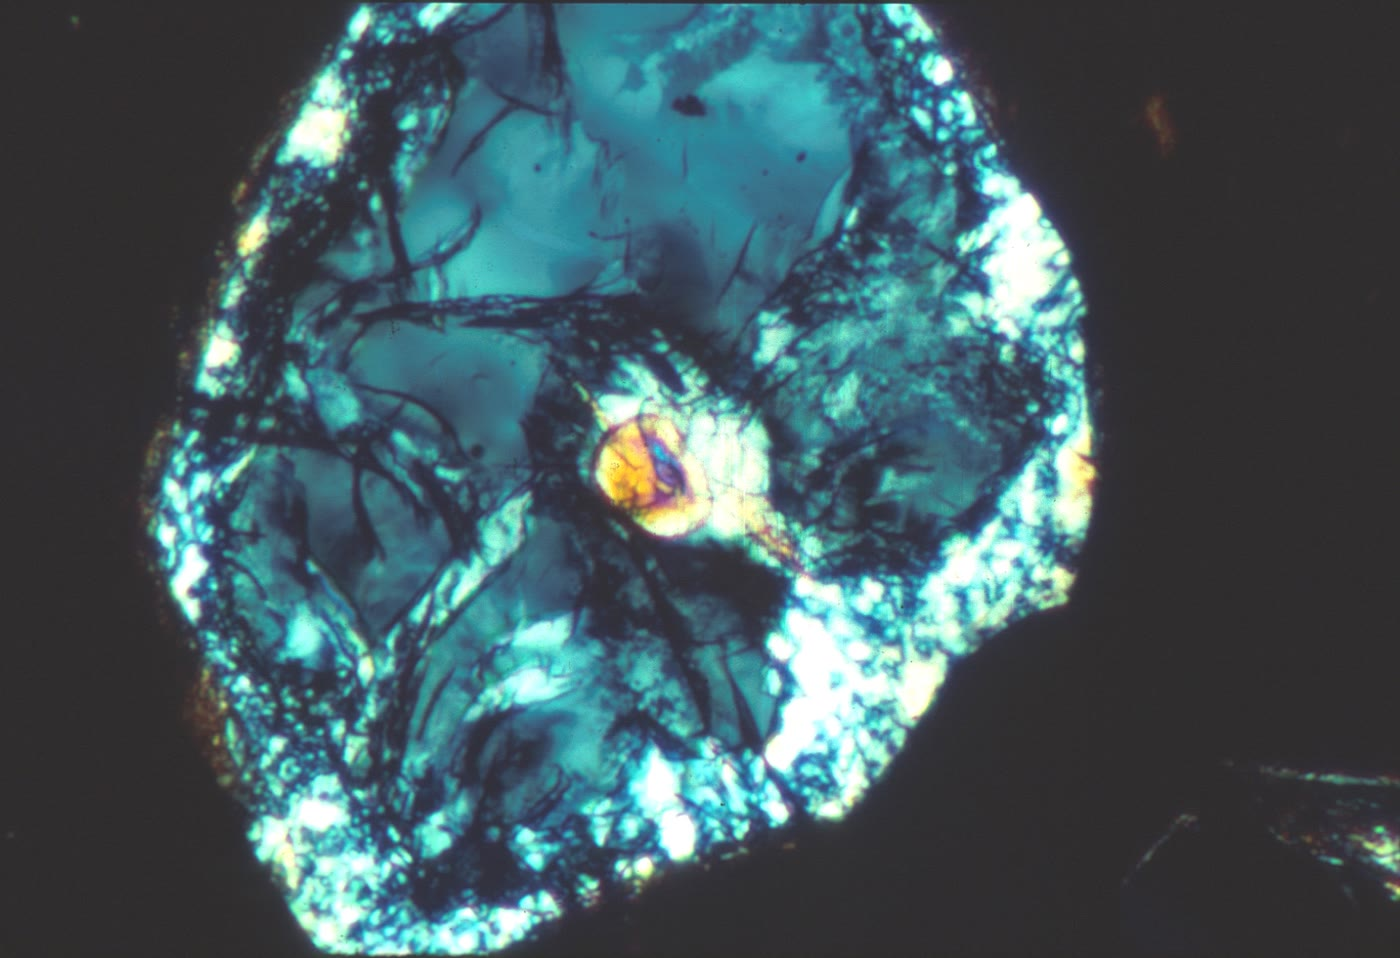
\includegraphics[width=0.62\linewidth]{images/book4/b2-11-coesite.jpg}
\par\smallskip{\small 榴辉岩中的柯石英，直径约 \qty{1}{mm}，薄片
正交偏光下观察：中央大颗粒为柯石英，周围一圈亮色小颗粒为
石英，是压力降低时由其生长出的；中央的小彩色颗粒为辉石包裹体。
照片：J.\,R. Smyth，CC BY-SA 1.0。}
\end{omfigure}

六年后，人们在哈萨克斯坦北部科克切塔夫地块的片麻岩、片岩及
石榴子石–辉石岩中发现了平均粒径为 \qty{12}{\micro m} 的金刚石，
包裹于石榴子石和锆石之中，二者使其免于转变为石墨：金刚石形成于
\qty{40}{kbar} 或更高的压强，以及 900 至 \qty{1000}{\celsius} 以上的温度。大陆地壳
虽然质轻，却可被拖入地下一百多千米。
% ledger: ss90:diamond

岩石如何\omterm{def:b2:pt-paths:exhumation}{折返}，由其“时钟”告诉我们。在阿尔卑斯山最深处俯冲的岩石中，
对连续阶段的榍石定年表明，一块钙硅酸盐岩曾达到约
\qty{3.5}{GPa}，时间为 $35.1 \pm \qty{0.9}{Ma}$；压强为 $1 \pm \qty{0.15}{GPa}$，时间为 $32.9 \pm
\qty{0.9}{Ma}$ 时，压强约为 0.4 至 \qty{0.5}{GPa}，时间为 $31.8 \pm \qty{0.5}{Ma}$。
平均\omterm{def:b2:pt-paths:exhumation}{折返速率}依次为 3.4 与 \qty{1.6}{cm.\text{年}^{-1}}，与板块速度相当：
岩石返回地表的速度与下沉时大致相当，远快于侵蚀
能将其剥露的速度。作者援引浮力机制，即轻质地壳在致密地幔中上升，
以及正断层作用，正断层使上覆岩石变薄。
% ledger: rh01:exhumation

\section{洋底变质作用}\label{sec:b2:pt-paths:ocean-floor}

\begin{definition}[洋底变质作用；蛇纹石化]\label{def:b2:pt-paths:ocean-floor}
称\emph{洋底变质作用}\index{洋底变质作用}为
扩张中心附近洋岩石圈的区域\omterm{def:b2:metamorphic-facies:metamorphism}{变质作用}，由热含水流体引起；
这些流体在陡峭的地温梯度下循环，重结晶一般不完全，
温度通常随深度增加。称\emph{蛇纹石化}\index{蛇纹石化}为
富橄榄石岩石水合生成蛇纹石的过程。
\end{definition}
% ledger: scmr:types

海水沿洋脊轴附近被吸入年轻的地壳，受热后与岩石发生反应，
然后又上升。途经的玄武岩不完全地重结晶，形成含水
矿物，温度范围很宽。水到达\omterm{def:b2:mantle-melting:peridotites}{橄榄岩}之处，例如
慢速扩张脊，那里地幔岩石抬升至海底，为
“失落之城”热液区等处的泉（见本科一年级分册）提供水源，橄榄石吸收水分：
\[
\ce{2 Mg2SiO4 + 3 H2O -> Mg3Si2O5(OH)4 + Mg(OH)2},
\]
摩尔体积分别为：镁橄榄石 43.65，蛇纹石 107.50，
水镁石为 \qty{24.63}{cm^3.mol^{-1}}，这说明了这一变化对岩石的影响：
\qty{87.30}{cm^3} 的橄榄石变为 \qty{132.13}{cm^3} 的固体，体积
增大 \qty{51}{\percent}，密度由 3.22 降至 \qty{2.54}{g.cm^{-3}}。岩石膨胀
并变轻，其结合的水也随板块俯冲而一同下沉。
% ledger: scmr:types, rh95:serpentine, kelley:lost-city, dick:ultraslow

\begin{inthelab}[解读石榴子石]
要解读 \omterm{def:b2:pt-paths:paths}{P--T 轨迹}，岩石学家首先沿石榴子石的中心切取薄片，
因为偏离中心的切片会错过核心部分。在显微镜下，包裹体
被逐一测绘：石英、黑云母、斜长石或蓝晶石的小颗粒，在石榴子石生长时被捕获，
有时呈线状排列，保存了岩石更早的面理。随后用电子
探针沿一条从核心到边缘的线测定成分，并绘出镁、铁、钙和锰的分布图，
以显示生长环带。每个环带都与同期生长的矿物配对：核心对应包裹体，
边缘对应与之接触的基质。温度计和压力计用于每一对矿物，
并在矿物允许时对环带定年，
\Cref{ch:b2:field-lab-methods-2} 介绍了这些仪器。
\end{inthelab}

\begin{omfigure}
\centering
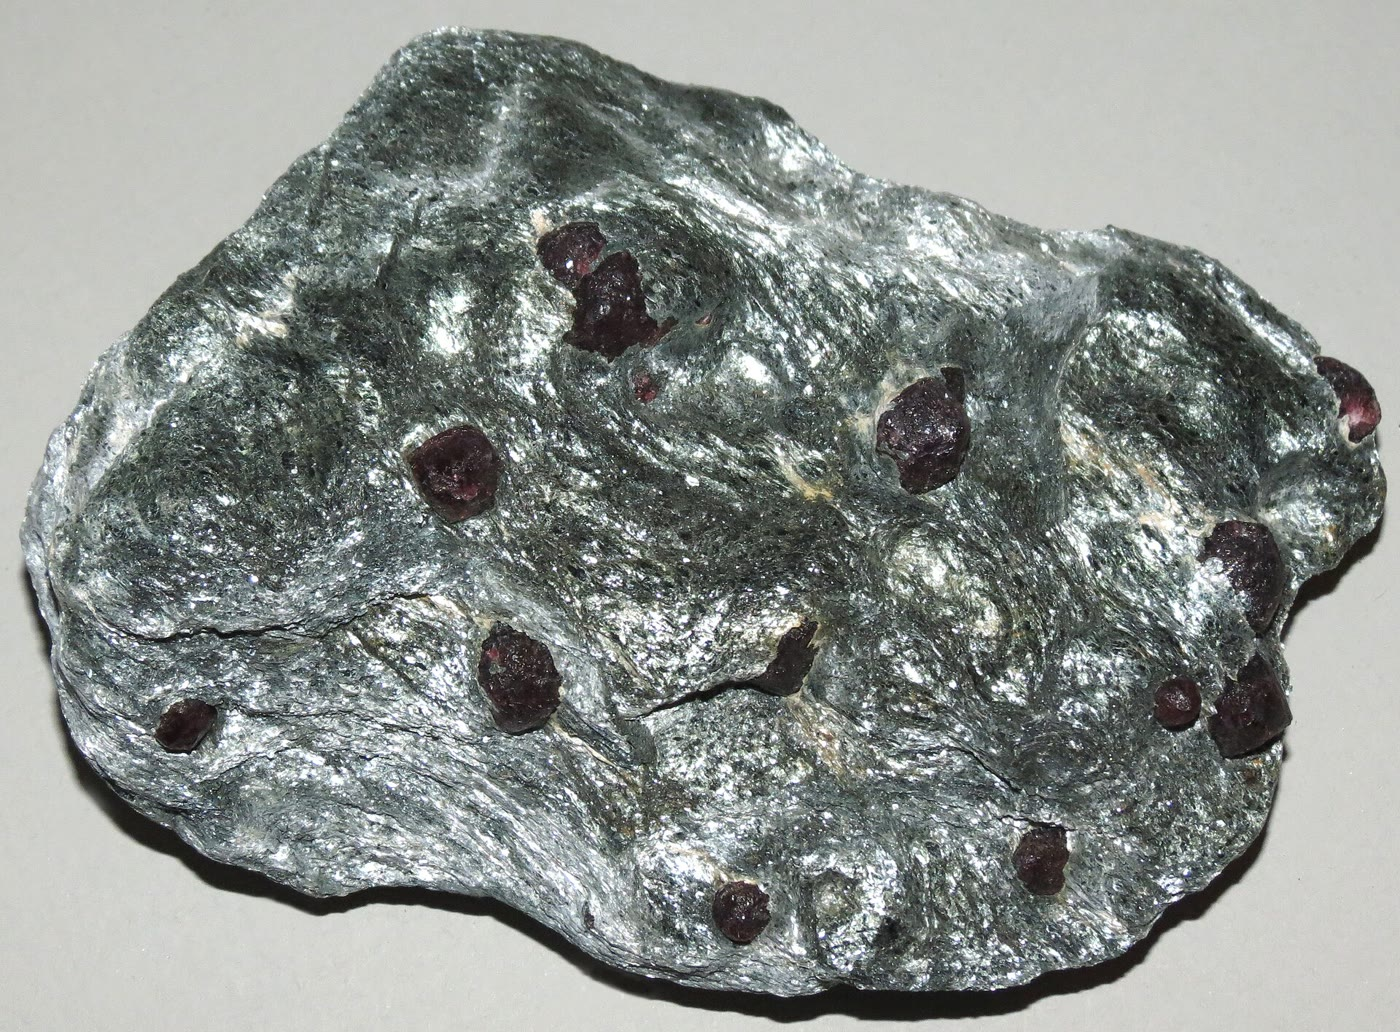
\includegraphics[width=0.62\linewidth]{images/book4/b2-11-garnet-schist.jpg}
\par\smallskip{\small 石榴子石片岩：深红色石榴子石晶体生长于
云母构成的面理状基质中。每颗石榴子石都能从核心到边缘保存
一段岩石路径的记录。照片：James St.~John，CC BY 2.0。}
\end{omfigure}

\section{练习}

\begin{exercise}[$\star$]\label{exo:b2:pt-paths:1}
沿一条公路采集的同一泥岩组的六个样品，分别含有：(A) 绿泥石、
白云母、石英；(B) 黑云母、绿泥石、白云母、石英；(C) 石榴子石、黑云母、
白云母、石英；(D) 十字石、石榴子石、黑云母、白云母、石英；(E) 蓝晶石、
十字石、黑云母、白云母、石英；(F) 夕线石、黑云母、白云母、石英。
(a) 各样品分别位于哪一\omterm{def:b2:pt-paths:barrovian}{巴罗带}？(b) 道路穿过多少条等变质线，
分别是哪些？(c) 为何仅知道等变质线不足以
绘制\omterm{def:b2:pt-paths:barrovian}{变质场梯度}？
\end{exercise}
% ledger: iugs:barrow

\begin{exercise}[$\star$]\label{exo:b2:pt-paths:2}
某石榴子石的 $X_{\text{Mg}} = 0.10$，$X_{\text{Fe}} = 0.80$，与之相邻的黑云母的
$X_{\text{Mg}} = 0.45$，$X_{\text{Fe}} = 0.50$。(a) 计算 $K_D$ 和 $\ln K_D$。
(b) 利用本章的标定式，计算压强为 \qty{5}{kbar} 和
\qty{7}{kbar} 时的温度。(c) 该结果是\omterm{def:b2:pt-paths:thermobarometry}{地质温度计}还是\omterm{def:b2:pt-paths:thermobarometry}{地质压力计}？
\end{exercise}
% ledger: h97:ideal, h97:fs-reaction

\begin{exercise}[$\star$]\label{exo:b2:pt-paths:3}
一\omterm{def:b2:metamorphic-facies:protoliths}{变泥质岩}给出 \qty{580}{\celsius} 与 \qty{6.0}{kbar}。(a) 若上覆岩石的平均密度为
\qty{2800}{kg.m^{-3}}（$g = \qty{9.81}{m.s^{-2}}$），该岩石曾位于多深处？(b) 据此，
以地表 \qty{10}{\celsius} 为起点，隐含的温度梯度为多少？(c) 实验所得的
蓝晶石 $=$ 夕线石平衡线经过 \qty{3.67}{kbar} 时的温度为
\qty{500}{\celsius}，经过 \qty{5.77}{kbar} 时温度为 \qty{600}{\celsius}：该岩石应含
哪种铝硅酸盐矿物？
\end{exercise}
% ledger: hm93:table11

\begin{exercise}[$\star$]\label{exo:b2:pt-paths:4}
对本章中写出的镁橄榄石\omterm{def:b2:pt-paths:ocean-floor}{蛇纹石化}反应：(a) 检验该方程的质量是否平衡，
已知摩尔质量分别为 140.693（镁橄榄石）、18.015（水），
277.112（蛇纹石）和 \qty{58.320}{g.mol^{-1}}（水镁石）；(b) 计算固体的
体积变化；(c) 计算橄榄石及各生成物的密度。
(d) 该变化对海底之下\omterm{def:b2:pt-paths:ocean-floor}{蛇纹石化}的\omterm{def:b2:mantle-melting:peridotites}{橄榄岩}有何影响？
\end{exercise}
% ledger: rh95:serpentine

\begin{exercise}[$\star\star$]\label{exo:b2:pt-paths:5}
用 \qty{2.07}{kbar} 下的四组实验标定\omterm{def:b2:pt-paths:thermobarometry}{地质温度计}，$\ln K_D =
-1.157$ 与 $-1.255$ 对应 \qty{799}{\celsius}，$-1.738$ 与 $-1.826$ 对应 \qty{550}{\celsius}。
(a) 对每一对取平均，求过两个平均值的直线 $\ln K_D = a/T + b$。
(b) 由此推出 $\Delta_r H$ 和 $\Delta_r S$，取 $\Delta_r V = \qty{0.311}{J.bar^{-1}}$。
(c) 比较你的标定与本章标定在
\qty{5}{kbar} 下 $K_D = 0.18$、$0.10$ 和 $0.30$ 时给出的温度，
对标定进行外推，你能得出什么结论？
\end{exercise}
% ledger: h97:fs-data, h97:ideal

\begin{exercise}[$\star\star$]\label{exo:b2:pt-paths:6}
(a) 由 \qty{298}{K} 下的摩尔体积（铁铝榴石 115.32、镁铝榴石 113.12、铁云母 154.30、
金云母 149.65、钙铝榴石 125.28、钙长石 100.79、蓝晶石 44.15、石英
\qty{22.69}{cm^3.mol^{-1}}），计算\omterm{def:b2:pt-paths:thermobarometry}{交换反应}与 GASP 反应的 $\Delta_r V$，
并与标定所用的值 \num{0.311} 和
\qty{-6.21}{J.bar^{-1}} 比较。(b) 对 $K_D = 0.18$，压强误差
\qty{1}{kbar} 会使温度改变多少开尔文？(c) 沿某岩石的 GASP 线（
$X_{\text{Ca}}/X_{\text{an}} = 0.20$），\qty{17}{K} 的温度误差会使
压强偏移多少巴？
\end{exercise}
% ledger: rh95:gb-gasp, rh95:al2sio5, h97:fs-reaction, kn88:gasp

\begin{exercise}[$\star\star$]\label{exo:b2:pt-paths:7}
在 \qty{600}{\celsius} 下，某石榴子石的 $X_{\text{Ca}} = 0.08$，与其相邻的斜长石
的 $X_{\text{an}} = 0.30$。(a) 计算 GASP 压强。(b) 取 $X_{\text{an}} =
0.35$ 重新计算。(c) 若平均密度为 \qty{2800}{kg.m^{-3}}，该岩石埋深多少？
\end{exercise}
% ledger: kn88:gasp

\begin{exercise}[$\star\star$]\label{exo:b2:pt-paths:8}
利用阿尔卑斯山最深处俯冲岩石的榍石年龄：约 \qty{3.5}{GPa} 对应
$35.1 \pm \qty{0.9}{Ma}$，\qty{1.0}{GPa} 对应 $32.9 \pm \qty{0.9}{Ma}$，\qty{0.45}{GPa} 对应
$31.8 \pm \qty{0.5}{Ma}$。(a) 取平均密度 \qty{3000}{kg.m^{-3}}，将
压强换算为深度。(b) 计算两个平均\omterm{def:b2:pt-paths:exhumation}{折返速率}，并与已发表的 3.4 和
\qty{1.6}{cm.\text{年}^{-1}} 比较。(c) 第一段时间
间隔的不确定度是多少？它允许的速率范围是什么？(d) 与加厚模型的
侵蚀速率 \qty{0.5}{mm.\text{年}^{-1}} 比较。
\end{exercise}
% ledger: rh01:exhumation

\begin{exercise}[$\star\star$]\label{exo:b2:pt-paths:9}
对 \qty{5}{kbar} 下的 $K_D = 0.18$，(a) 由命题计算 $\partial T/\partial\ln K_D$ 和
$\partial T/\partial P$；(b) 取 $\sigma_{\ln K_D} = 0.05$（即 $K_D$ 的
\qty{5}{\percent} 误差）和 $\sigma_P = \qty{1}{kbar}$，计算 $\sigma_T$。
(c) 哪一项误差占主导？请与最佳标定所声称的
\qty{25}{\celsius} 不确定度相比较。
\end{exercise}
% ledger: h97:ideal

\begin{exercise}[$\star\star\star$]\label{exo:b2:pt-paths:10}
某石榴子石边缘的 $X_{\text{Mg}} = 0.10$、$X_{\text{Fe}} = 0.75$、$X_{\text{Ca}} = 0.07$；
基质黑云母的 $X_{\text{Mg}} = 0.42$、$X_{\text{Fe}} = 0.52$；斜长石的
$X_{\text{an}} = 0.25$。(a) 应用本章方法，从 \qty{6}{kbar} 出发，
直至温度变化小于 \qty{1}{K}。(b) 该岩石应含
哪种铝硅酸盐？（采用\cref{exo:b2:pt-paths:3}中的实验线）(c) 为什么\omterm{def:b2:pt-paths:thermobarometry}{地质压力计}必须采用
实际存在的铝硅酸盐？
\end{exercise}
% ledger: h97:ideal, kn88:gasp, hm93:table11

\begin{exercise}[$\star\star\star$]\label{exo:b2:pt-paths:11}
取 $\kappa = \qty{1e-6}{m^2.s^{-1}}$，(a) 计算命题中的
弛豫时间，分别取 $L = \qty{35}{km}$ 与 $L = \qty{70}{km}$。(b) 模型侵蚀
\qty{35}{km} 需要 7000 万年；将该时间与(a)中的两个时间比较。(c) 由这些时间说明，
为何模型中的岩石先达到压力峰、后达到
热峰。(d) 若侵蚀快 10 倍，轨迹会有何变化？
\end{exercise}
% ledger: delaney:conductivity, et84:ptt

\begin{exercise}[$\star\star\star$]\label{exo:b2:pt-paths:12}
设地壳厚 \qty{35}{km}、密度为 \qty{2800}{kg.m^{-3}}，其下为
密度为 \qty{3300}{kg.m^{-3}} 的地幔。(a) 压强达到 \qty{28}{kbar}，即
多拉·马伊拉柯石英的最低压强时，深度为多少？(b) 对科克切塔夫金刚石所需的 \qty{40}{kbar}，深度又为多少？
(c) 在 (a) 所求深度处取 \qty{700}{\celsius}，隐含的平均梯度是多少，它落在哪一
类\omterm{def:b2:pt-paths:series}{变质系列}中？(d) 以 \qty{3.4}{cm.\text{年}^{-1}} 的速率，从
(a) 所求深度回升至 \qty{35}{km} 需要多长时间？
\end{exercise}
% ledger: chopin84:coesite, ss90:diamond, rh01:exhumation

\section{问题：一颗石榴子石的历程}

\begin{problem}[{周末问题——一块片岩的温压法、轨迹与
折返速率}]
\label{pb:b2:pt-paths:1}
一块蓝晶石–石榴子石–黑云母片岩中含有带核部和边缘的石榴子石。核部包裹着
黑云母、斜长石和蓝晶石；边缘与
基质中的黑云母和斜长石相接。石榴子石周围部分蓝晶石被夕线石取代，石榴子石的
边缘生长了一些绿泥石。分析结果如下：
\begin{center}
\small
\begin{tabular}{@{}lccc@{}}
\hline
 & $X_{\text{Mg}}$ & $X_{\text{Fe}}$ & $X_{\text{Ca}}$ 或 $X_{\text{an}}$\\
\hline
石榴子石核部 & 0.080 & 0.760 & 0.050\\
核部包裹的黑云母 & 0.40 & 0.58 &——\\
核部包裹的斜长石 &——&——& 0.25\\
石榴子石边缘 & 0.120 & 0.720 & 0.060\\
基质黑云母 & 0.46 & 0.53 &——\\
基质斜长石 &——&——& 0.28\\
\hline
\end{tabular}
\end{center}
采用本章的石榴子石–黑云母\omterm{def:b2:pt-paths:thermobarometry}{地质温度计}和 GASP \omterm{def:b2:pt-paths:thermobarometry}{地质压力计}（理想混合），
$R = \qty{8.314}{J.mol^{-1}.K^{-1}}$，$g = \qty{9.81}{m.s^{-2}}$，平均密度为
\qty{2800}{kg.m^{-3}}（岩石之上），并将各比值保留四位小数。

\noindent\textbf{第一部分——温度。}
\begin{enumerate}
\item 计算石榴子石核部及包裹黑云母中的 $X_{\text{Mg}}/X_{\text{Fe}}$，
再求核部的 $K_D$ 与 $\ln K_D$。
\item 对边缘及基质黑云母做同样计算。
\item 计算压力为 \qty{6}{kbar} 时核部的温度。
\item 计算压力为 \qty{6}{kbar} 时边缘的温度。
\item 若压力误差为 \qty{1}{kbar}，这些温度将变化多少开尔文？
\item 为何核部与包裹黑云母成对，而边缘与基质
黑云母成对？
\end{enumerate}

\noindent\textbf{第二部分——压强。}
\begin{enumerate}[resume]
\item 求 GASP 反应在两个温度下的端元压强 $P_0$，
即问题~3 和问题~4 中的温度。
\item 计算问题~3 温度下核部的 GASP 压强。
\item 计算问题~4 温度下边缘的 GASP 压强。
\item 以问题~9 的压强重新计算边缘的温度，再
以该温度求其压强，然后再算一次温度。给出边缘的温度
与压强。
\item 对核部同样做一次。为何它的变化如此之小？
\item 将核部和边缘的压强换算为深度。
\item 实验测定的蓝晶石 $=$ 夕线石分界线经过 3.67、5.77 和
\qty{7.86}{kbar}，对应温度 500、600 和 \qty{700}{\celsius}。哪种铝硅酸盐稳定
于核部生长时与边缘生长时？核部的蓝晶石是否相符？
\end{enumerate}

\noindent\textbf{第三部分——轨迹。}
\begin{enumerate}[resume]
\item 从核部到边缘，温度与压强各变化了多少？
石榴子石生长于\omterm{def:b2:pt-paths:paths}{进变质轨迹}还是\omterm{def:b2:pt-paths:paths}{退变质轨迹}上？
\item 夕线石环绕石榴子石替代蓝晶石。在边缘温度下，
岩石须降至低于多大压强，才会发生这种替代？
边缘生长之后，岩石经历了什么？
\item 绿泥石生长于石榴子石边缘。它记录的是轨迹的哪一段？
\item 画出轨迹：核部、边缘、夕线石、绿泥石。它是顺时针还是逆时针？
哪一个峰期先出现？
\item 本章增厚模型使岩石达到的热峰期，温度为
\qty{593}{\celsius}、压强为 \qty{7.8}{kbar}。片岩的轨迹是否属同一类型？
\end{enumerate}

\noindent\textbf{第四部分——速率。}
\begin{enumerate}[resume]
\item 石榴子石边缘给出钐–钕年龄 $412.0 \pm \qty{1.5}{Ma}$，
取作峰期年龄；基质白云母给出氩年龄 $398.0 \pm
\qty{1.0}{Ma}$，即岩石冷却穿过 \qty{405}{\celsius} 的时刻。计算
两者之间的平均冷却速率。
\item 封闭温度 \qty{405}{\celsius} 假设冷却速率为
\qty{10}{\celsius}，每百万年。问题~19 的速率需要
更高还是更低的封闭温度？为什么？
\item 在 \qty{398}{Ma} 时，取地温线，梯度为
\qty{30}{\celsius\per\km}，自地表 \qty{10}{\celsius} 起算。白云母在何深度封闭？
\item 从峰期到白云母封闭期间，岩石上升了多远？
\item 该时间间隔的不确定度是多少？
\item 计算从峰期到白云母封闭的平均\omterm{def:b2:pt-paths:exhumation}{折返速率}，单位为
毫米每年，保留一位小数：这是本题的关键数值。
\end{enumerate}
\end{problem}
% ledger: h97:ideal, h97:fs-reaction, kn88:gasp, hm93:table11, h09:muscovite, scmr:ptt, et84:ptt
